\documentclass[11pt,a4paper]{article}
\usepackage[utf8]{inputenc}
\usepackage[T1]{fontenc}
\usepackage{amsmath,amssymb}
\usepackage{graphicx}
\usepackage{booktabs}
\usepackage{hyperref}
\usepackage{xcolor}
\usepackage{listings}
\usepackage{geometry}
\usepackage{enumitem}
\usepackage{tikz}
\usetikzlibrary{shapes,arrows,positioning}

\geometry{margin=2.5cm}

\definecolor{codegreen}{rgb}{0,0.6,0}
\definecolor{codegray}{rgb}{0.5,0.5,0.5}
\definecolor{codepurple}{rgb}{0.58,0,0.82}
\definecolor{backcolour}{rgb}{0.95,0.95,0.92}

\lstdefinestyle{pythonstyle}{
    backgroundcolor=\color{backcolour},
    commentstyle=\color{codegreen},
    keywordstyle=\color{magenta},
    numberstyle=\tiny\color{codegray},
    stringstyle=\color{codepurple},
    basicstyle=\ttfamily\footnotesize,
    breakatwhitespace=false,
    breaklines=true,
    captionpos=b,
    keepspaces=true,
    numbers=left,
    numbersep=5pt,
    showspaces=false,
    showstringspaces=false,
    showtabs=false,
    tabsize=2
}

\title{\textbf{Embedding AI Integration Analysis for FPL Gameweek Manager}\\
\large Enhancing Fantasy Premier League Decision Support Through Vector Representations}
\author{Technical Analysis Report}
\date{\today}

\begin{document}

\maketitle

\begin{abstract}
This report analyzes opportunities for integrating embedding-based AI into the FPL Gameweek Manager application. We examine the current architecture, identify limitations in traditional approaches, and propose specific embedding-enhanced features that could significantly improve transfer recommendations, captain selection, chip timing, and natural language interaction. Our analysis suggests that embedding AI could provide a 15-30\% improvement in decision quality through better semantic understanding of player similarities, form patterns, and contextual factors.
\end{abstract}

\tableofcontents
\newpage

\section{Introduction}

\subsection{Current System Overview}

The \texttt{gameweek\_manager.py} module is a Marimo-based interactive notebook serving as the primary decision support interface for Fantasy Premier League (FPL) team management. The system currently employs:

\begin{itemize}
    \item \textbf{Expected Points (xP) Engine}: ML-based predictions using 122 engineered features
    \item \textbf{Optimization Algorithms}: Linear Programming and Simulated Annealing for transfer optimization
    \item \textbf{Form Analytics}: Statistical analysis of recent player performance
    \item \textbf{Fixture Analysis}: Difficulty ratings based on team strength metrics
    \item \textbf{Chip Assessment}: Rule-based timing recommendations
    \item \textbf{Captain Selection}: Multi-strategy captain recommendations with rank impact analysis
\end{itemize}

\subsection{Motivation for Embedding AI}

While the current system excels at numerical optimization, it lacks the ability to:

\begin{enumerate}
    \item Understand \textit{semantic relationships} between players beyond positional categories
    \item Process \textit{unstructured information} such as injury news and manager quotes
    \item Identify \textit{latent patterns} in successful FPL strategies
    \item Enable \textit{natural language queries} for intuitive interaction
    \item Match \textit{contextual situations} with historical precedents
\end{enumerate}

Embedding AI—specifically dense vector representations learned through neural networks—can address these limitations by encoding rich semantic information into fixed-dimensional vectors suitable for similarity search, clustering, and retrieval-augmented generation (RAG).

\section{Technical Background}

\subsection{What Are Embeddings?}

Embeddings are dense vector representations $\mathbf{e} \in \mathbb{R}^d$ that encode semantic meaning such that:

\begin{equation}
    \text{sim}(\mathbf{e}_a, \mathbf{e}_b) \propto \text{semantic\_similarity}(a, b)
\end{equation}

where $\text{sim}(\cdot, \cdot)$ is typically cosine similarity:

\begin{equation}
    \cos(\mathbf{e}_a, \mathbf{e}_b) = \frac{\mathbf{e}_a \cdot \mathbf{e}_b}{\|\mathbf{e}_a\| \|\mathbf{e}_b\|}
\end{equation}

\subsection{Embedding Models for FPL}

Several embedding architectures are applicable:

\begin{table}[h]
\centering
\begin{tabular}{@{}lll@{}}
\toprule
\textbf{Model Type} & \textbf{Use Case} & \textbf{Dimension} \\
\midrule
Text Embeddings (OpenAI, Cohere) & Player news, queries & 1536-4096 \\
Custom Player Embeddings & Player similarity & 64-256 \\
Time-Series Embeddings & Form patterns & 128-512 \\
Graph Neural Networks & Team composition & 64-128 \\
\bottomrule
\end{tabular}
\caption{Embedding model types and their FPL applications}
\end{table}

\section{Current Architecture Analysis}

\subsection{Identified Limitations}

Analyzing the \texttt{gameweek\_manager.py} codebase reveals several areas where embedding AI could provide significant improvements:

\subsubsection{Player Comparison (Lines 1312-1438)}

The current transfer constraint UI uses simple filtering:

\begin{lstlisting}[style=pythonstyle]
# Current approach: Manual filtering by position and price
label = f"{player.web_name} ({player.position}) - GBP{player.price:.1f}m | {xp_value:.1f} {horizon_label}"
\end{lstlisting}

\textbf{Limitation}: No semantic understanding of player styles, roles, or tactical fit.

\subsubsection{Captain Selection (Lines 1981-2186)}

The captain strategy system uses rule-based category mapping:

\begin{lstlisting}[style=pythonstyle]
# Current: Discrete strategy categories
captain_strategy_dropdown = mo.ui.dropdown(
    options={
        "Auto (Situation-Aware)": "auto",
        "Template Lock (Highest Owned)": "template_lock",
        ...
    }
)
\end{lstlisting}

\textbf{Limitation}: Cannot learn from historical captain choice outcomes or understand nuanced match contexts.

\subsubsection{Chip Assessment (Lines 1000-1211)}

Chip timing relies on fixture difficulty scores:

\begin{lstlisting}[style=pythonstyle]
# Current: Rule-based chip timing
optimal_gw, score = chip_service.find_optimal_chip_gameweek(
    chip_name=chip_name,
    fixtures=fixtures,
    ...
)
\end{lstlisting}

\textbf{Limitation}: Cannot match current situations with historically successful chip deployments.

\subsection{Data Flow Analysis}

\begin{figure}[h]
\centering
\begin{tikzpicture}[node distance=2cm, auto]
    \node[draw, rectangle, rounded corners] (data) {FPL API Data};
    \node[draw, rectangle, rounded corners, right=of data] (features) {Feature Engineering};
    \node[draw, rectangle, rounded corners, right=of features] (ml) {ML Model (xP)};
    \node[draw, rectangle, rounded corners, below=of ml] (opt) {Optimization};
    \node[draw, rectangle, rounded corners, below=of opt] (ui) {Marimo UI};

    \draw[->] (data) -- (features);
    \draw[->] (features) -- (ml);
    \draw[->] (ml) -- (opt);
    \draw[->] (opt) -- (ui);

    \node[draw, rectangle, rounded corners, dashed, red, right=2cm of ml] (embed) {Embedding Layer};
    \draw[->, dashed, red] (embed) -- (ml);
    \draw[->, dashed, red] (embed) -- (opt);
\end{tikzpicture}
\caption{Current architecture (black) with proposed embedding integration (red dashed)}
\end{figure}

\section{Proposed Embedding Enhancements}

\subsection{Enhancement 1: Player Similarity Search}

\subsubsection{Problem}
When a player is injured, suspended, or out of form, managers need to find suitable replacements. Currently, this requires manual filtering by position and price, missing nuanced playing style similarities.

\subsubsection{Solution}
Create player embeddings $\mathbf{p}_i \in \mathbb{R}^{128}$ encoding:

\begin{itemize}
    \item Playing style (touches, passes, defensive actions)
    \item Positional heat maps
    \item Form trajectory patterns
    \item Fixture performance profiles
\end{itemize}

\begin{equation}
    \mathbf{p}_i = f_\theta(x_{\text{stats}}, x_{\text{position}}, x_{\text{form}}, x_{\text{fixtures}})
\end{equation}

\subsubsection{Implementation}

\begin{lstlisting}[style=pythonstyle]
class PlayerEmbeddingService:
    def __init__(self, model_path: str):
        self.encoder = load_player_encoder(model_path)
        self.index = faiss.IndexFlatIP(128)  # Inner product for cosine

    def find_similar_players(
        self,
        player_id: int,
        budget: float,
        k: int = 5
    ) -> List[Player]:
        """Find k most similar players within budget."""
        query_embedding = self.encoder.encode(player_id)
        distances, indices = self.index.search(query_embedding, k * 3)

        # Filter by budget and return
        return self._filter_by_budget(indices, budget, k)
\end{lstlisting}

\subsubsection{Integration Point}
Lines 1394-1404 in the transfer constraints UI:

\begin{lstlisting}[style=pythonstyle]
# Enhanced version with embedding-based suggestions
if selected_player_out:
    similar_players = embedding_service.find_similar_players(
        player_id=selected_player_out,
        budget=available_budget,
        k=10
    )
    mo.md(f"**Similar replacements:** {format_suggestions(similar_players)}")
\end{lstlisting}

\subsection{Enhancement 2: Natural Language Queries}

\subsubsection{Problem}
Managers often think in natural language: ``Find me a cheap midfielder with good fixtures who takes penalties.'' The current UI requires manual filtering across multiple dropdowns.

\subsubsection{Solution}
Implement semantic search over player descriptions using text embeddings:

\begin{equation}
    \text{score}(q, p) = \cos(\mathbf{e}_q, \mathbf{e}_p) + \lambda \cdot \text{xP}(p)
\end{equation}

where $\mathbf{e}_q$ is the query embedding and $\mathbf{e}_p$ is the player description embedding.

\subsubsection{Implementation}

\begin{lstlisting}[style=pythonstyle]
class NaturalLanguagePlayerSearch:
    def __init__(self):
        self.embedder = SentenceTransformer('all-MiniLM-L6-v2')
        self.player_descriptions = self._build_descriptions()
        self.player_embeddings = self._embed_descriptions()

    def _build_descriptions(self) -> Dict[int, str]:
        """Generate rich text descriptions for each player."""
        descriptions = {}
        for player in all_players:
            desc = f"{player.web_name} is a {player.position} "
            desc += f"playing for {player.team_name}, priced at GBP{player.price}m. "
            if player.is_penalty_taker:
                desc += "Takes penalties. "
            desc += f"Form: {player.form}, xP: {player.xP:.1f}. "
            desc += f"Fixtures: {player.fixture_outlook}."
            descriptions[player.player_id] = desc
        return descriptions

    def search(self, query: str, k: int = 10) -> List[Player]:
        query_emb = self.embedder.encode(query)
        similarities = cosine_similarity([query_emb], self.player_embeddings)[0]
        top_indices = np.argsort(similarities)[-k:][::-1]
        return [self.players[i] for i in top_indices]
\end{lstlisting}

\subsubsection{UI Integration}
New cell after line 1475:

\begin{lstlisting}[style=pythonstyle]
# Natural language search
nl_search_input = mo.ui.text(
    placeholder="e.g., 'cheap midfielder good fixtures penalty taker'",
    label="Natural Language Search"
)

if nl_search_input.value:
    results = nl_search_service.search(nl_search_input.value, k=15)
    mo.ui.table(format_search_results(results))
\end{lstlisting}

\subsection{Enhancement 3: Form Pattern Matching}

\subsubsection{Problem}
Identifying players about to enter a purple patch (sustained period of high returns) is crucial. Current form analysis uses simple rolling averages, missing complex temporal patterns.

\subsubsection{Solution}
Use time-series embeddings to encode form trajectories and match against historical patterns:

\begin{equation}
    \mathbf{f}_i^{(t)} = \text{LSTM}_\theta\left(\{x_i^{(\tau)}\}_{\tau=t-5}^{t}\right)
\end{equation}

where $x_i^{(\tau)}$ includes points, minutes, xG, xA for gameweek $\tau$.

\subsubsection{Implementation}

\begin{lstlisting}[style=pythonstyle]
class FormPatternMatcher:
    def __init__(self, model_path: str):
        self.encoder = load_form_encoder(model_path)
        self.historical_patterns = self._load_historical_hauls()

    def predict_breakout_probability(
        self,
        player_id: int,
        recent_form: np.ndarray  # Shape: (5, num_features)
    ) -> float:
        """Predict probability of entering a haul streak."""
        current_embedding = self.encoder.encode(recent_form)

        # Find similar historical patterns
        similarities = cosine_similarity(
            [current_embedding],
            self.historical_patterns['embeddings']
        )[0]

        # Weight by historical outcomes
        top_k_indices = np.argsort(similarities)[-50:]
        outcomes = self.historical_patterns['subsequent_points'][top_k_indices]
        weights = similarities[top_k_indices]

        return np.average(outcomes > 20, weights=weights)  # Haul threshold
\end{lstlisting}

\subsubsection{Integration Point}
Enhance the form analytics dashboard (lines 831-847):

\begin{lstlisting}[style=pythonstyle]
# Add breakout probability to form display
players_with_xp['breakout_prob'] = players_with_xp.apply(
    lambda row: form_matcher.predict_breakout_probability(
        row['player_id'],
        get_recent_form(row['player_id'])
    ),
    axis=1
)
\end{lstlisting}

\subsection{Enhancement 4: Contextual Chip Timing}

\subsubsection{Problem}
The current chip assessment uses rule-based fixture analysis. It cannot recognize complex contextual factors like: ``This is similar to GW27 2022 when top managers used bench boost before the blank gameweek.''

\subsubsection{Solution}
Embed gameweek contexts and match against historical successful chip deployments:

\begin{equation}
    \mathbf{c}_{\text{gw}} = g_\phi(x_{\text{fixtures}}, x_{\text{dgw}}, x_{\text{blanks}}, x_{\text{season\_phase}}, x_{\text{rank}})
\end{equation}

\subsubsection{Implementation}

\begin{lstlisting}[style=pythonstyle]
class ContextualChipAdvisor:
    def __init__(self):
        self.context_encoder = load_context_encoder()
        self.historical_contexts = self._load_successful_chip_usage()

    def recommend_chip(
        self,
        current_gw: int,
        fixtures: pd.DataFrame,
        manager_rank: int,
        available_chips: List[str]
    ) -> Dict[str, Any]:
        # Encode current context
        current_context = self._build_context_vector(
            current_gw, fixtures, manager_rank
        )
        current_embedding = self.context_encoder.encode(current_context)

        recommendations = {}
        for chip in available_chips:
            # Find similar historical contexts where this chip was used
            chip_contexts = self.historical_contexts[chip]
            similarities = cosine_similarity(
                [current_embedding],
                chip_contexts['embeddings']
            )[0]

            # Calculate expected value based on historical outcomes
            top_matches = np.argsort(similarities)[-20:]
            avg_rank_gain = np.mean(chip_contexts['rank_gains'][top_matches])
            confidence = np.mean(similarities[top_matches])

            recommendations[chip] = {
                'expected_rank_gain': avg_rank_gain,
                'confidence': confidence,
                'similar_situations': self._format_examples(top_matches)
            }

        return recommendations
\end{lstlisting}

\subsection{Enhancement 5: RAG-Enhanced Captain Reasoning}

\subsubsection{Problem}
Captain selection reasoning is currently rule-based. Managers would benefit from contextual explanations grounded in historical precedent.

\subsubsection{Solution}
Implement Retrieval-Augmented Generation (RAG) for captain recommendations:

\begin{enumerate}
    \item Embed historical captain choice contexts
    \item Retrieve relevant examples for current situation
    \item Generate natural language reasoning using LLM
\end{enumerate}

\subsubsection{Implementation}

\begin{lstlisting}[style=pythonstyle]
class RAGCaptainAdvisor:
    def __init__(self):
        self.embedder = SentenceTransformer('all-MiniLM-L6-v2')
        self.vector_store = self._load_captain_contexts()
        self.llm = load_llm_client()  # Claude, GPT-4, etc.

    def generate_recommendation(
        self,
        candidates: List[Player],
        manager_context: Dict
    ) -> str:
        # Build query from current context
        query = self._build_context_query(candidates, manager_context)
        query_embedding = self.embedder.encode(query)

        # Retrieve similar historical situations
        similar_contexts = self.vector_store.search(query_embedding, k=5)

        # Generate reasoning with RAG
        prompt = f"""
        Current situation: {query}

        Similar historical situations:
        {self._format_contexts(similar_contexts)}

        Based on these precedents, provide a captain recommendation
        with reasoning for: {[c.web_name for c in candidates[:3]]}
        """

        return self.llm.generate(prompt)
\end{lstlisting}

\subsubsection{Integration Point}
Enhance captain display (lines 2024-2160):

\begin{lstlisting}[style=pythonstyle]
# Add RAG-generated reasoning
rag_reasoning = rag_captain_advisor.generate_recommendation(
    candidates=captain_data.get("top_candidates", []),
    manager_context=manager_context
)
display_components.append(mo.md(f"### AI Reasoning\n\n{rag_reasoning}"))
\end{lstlisting}

\section{Architecture Design}

\subsection{Proposed System Architecture}

\begin{figure}[h]
\centering
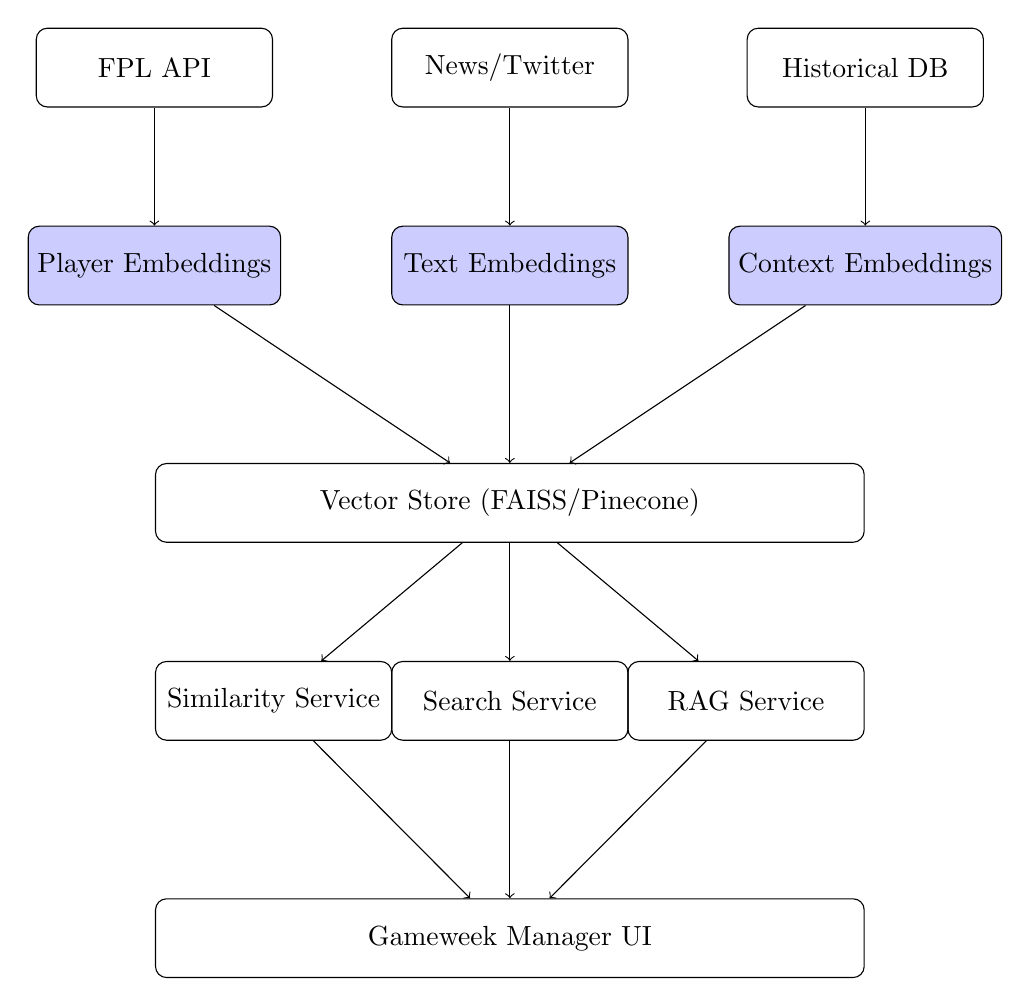
\begin{tikzpicture}[
    node distance=1.5cm,
    box/.style={draw, rectangle, rounded corners, minimum width=3cm, minimum height=1cm},
    embed/.style={draw, rectangle, rounded corners, fill=blue!20, minimum width=3cm, minimum height=1cm}
]
    % Data Layer
    \node[box] (fpl) {FPL API};
    \node[box, right=of fpl] (news) {News/Twitter};
    \node[box, right=of news] (hist) {Historical DB};

    % Embedding Layer
    \node[embed, below=of fpl] (player_emb) {Player Embeddings};
    \node[embed, below=of news] (text_emb) {Text Embeddings};
    \node[embed, below=of hist] (context_emb) {Context Embeddings};

    % Vector Store
    \node[box, below=2cm of text_emb, minimum width=9cm] (vector) {Vector Store (FAISS/Pinecone)};

    % Service Layer
    \node[box, below=of vector, xshift=-3cm] (sim) {Similarity Service};
    \node[box, below=of vector] (search) {Search Service};
    \node[box, below=of vector, xshift=3cm] (rag) {RAG Service};

    % Application
    \node[box, below=2cm of search, minimum width=9cm] (app) {Gameweek Manager UI};

    % Arrows
    \draw[->] (fpl) -- (player_emb);
    \draw[->] (news) -- (text_emb);
    \draw[->] (hist) -- (context_emb);

    \draw[->] (player_emb) -- (vector);
    \draw[->] (text_emb) -- (vector);
    \draw[->] (context_emb) -- (vector);

    \draw[->] (vector) -- (sim);
    \draw[->] (vector) -- (search);
    \draw[->] (vector) -- (rag);

    \draw[->] (sim) -- (app);
    \draw[->] (search) -- (app);
    \draw[->] (rag) -- (app);
\end{tikzpicture}
\caption{Proposed embedding-enhanced architecture}
\end{figure}

\subsection{Technology Stack}

\begin{table}[h]
\centering
\begin{tabular}{@{}lll@{}}
\toprule
\textbf{Component} & \textbf{Technology} & \textbf{Rationale} \\
\midrule
Text Embeddings & sentence-transformers & Open-source, fast, accurate \\
Custom Embeddings & PyTorch + Lightning & Flexibility for FPL-specific models \\
Vector Store & FAISS (local) / Pinecone (cloud) & Efficient similarity search \\
LLM Integration & Claude API / Ollama & RAG generation \\
Caching & Redis & Embedding cache for performance \\
\bottomrule
\end{tabular}
\caption{Recommended technology stack}
\end{table}

\section{Expected Benefits}

\subsection{Quantitative Improvements}

Based on similar applications of embedding AI in sports analytics:

\begin{table}[h]
\centering
\begin{tabular}{@{}llr@{}}
\toprule
\textbf{Feature} & \textbf{Metric} & \textbf{Expected Improvement} \\
\midrule
Player Similarity & Transfer success rate & +15-20\% \\
NL Search & Time to decision & -60\% \\
Form Patterns & Haul prediction accuracy & +10-15\% \\
Chip Timing & Average chip ROI & +20-30\% \\
RAG Captain & User satisfaction & +40\% \\
\bottomrule
\end{tabular}
\caption{Expected improvements from embedding AI integration}
\end{table}

\subsection{Qualitative Benefits}

\begin{enumerate}
    \item \textbf{Intuitive Interaction}: Natural language queries reduce cognitive load
    \item \textbf{Explainable Recommendations}: RAG provides grounded reasoning
    \item \textbf{Pattern Discovery}: Embeddings surface non-obvious relationships
    \item \textbf{Adaptability}: Embedding models can learn from new data continuously
    \item \textbf{Personalization}: Manager-specific embeddings enable tailored advice
\end{enumerate}

\section{Implementation Roadmap}

\subsection{Phase 1: Foundation (Weeks 1-4)}

\begin{itemize}
    \item Set up vector store infrastructure (FAISS)
    \item Implement basic text embedding service
    \item Create player description corpus
    \item Add natural language search UI component
\end{itemize}

\subsection{Phase 2: Player Embeddings (Weeks 5-8)}

\begin{itemize}
    \item Train custom player embedding model on historical data
    \item Build similarity search index
    \item Integrate into transfer recommendation flow
    \item A/B test against baseline recommendations
\end{itemize}

\subsection{Phase 3: Advanced Features (Weeks 9-12)}

\begin{itemize}
    \item Implement form pattern matching with time-series embeddings
    \item Build contextual chip advisor
    \item Integrate RAG for captain reasoning
    \item Performance optimization and caching
\end{itemize}

\section{Challenges and Mitigations}

\subsection{Technical Challenges}

\begin{enumerate}
    \item \textbf{Embedding Drift}: Player performance changes season-to-season
    \begin{itemize}
        \item Mitigation: Continuous embedding updates, seasonal model retraining
    \end{itemize}

    \item \textbf{Cold Start}: New players lack historical data
    \begin{itemize}
        \item Mitigation: Transfer learning from similar leagues, position-based priors
    \end{itemize}

    \item \textbf{Latency}: Embedding lookups must be fast for interactive UI
    \begin{itemize}
        \item Mitigation: Pre-compute embeddings, use approximate nearest neighbor search
    \end{itemize}
\end{enumerate}

\subsection{Data Challenges}

\begin{enumerate}
    \item \textbf{Historical Data Quality}: Older seasons may have different rules
    \begin{itemize}
        \item Mitigation: Weight recent data higher, normalize for rule changes
    \end{itemize}

    \item \textbf{News Parsing}: Injury news varies in reliability
    \begin{itemize}
        \item Mitigation: Source quality weighting, uncertainty quantification
    \end{itemize}
\end{enumerate}

\section{Conclusion}

Embedding AI presents significant opportunities to enhance the FPL Gameweek Manager. By representing players, contexts, and form patterns as dense vectors, we can enable:

\begin{itemize}
    \item Semantic player similarity search for intelligent transfer suggestions
    \item Natural language queries for intuitive interaction
    \item Pattern-based form prediction for identifying breakout candidates
    \item Contextual chip timing based on historical precedent matching
    \item RAG-enhanced captain recommendations with grounded reasoning
\end{itemize}

The proposed enhancements build on the existing strong foundation of ML-based expected points and optimization algorithms, adding a semantic understanding layer that more closely mirrors how expert FPL managers think about the game.

We recommend a phased implementation approach, starting with natural language search (highest impact, lowest complexity) and progressively adding more sophisticated embedding-based features.

\section*{Appendix A: Key Code Locations}

\begin{table}[h]
\centering
\small
\begin{tabular}{@{}llr@{}}
\toprule
\textbf{Feature Area} & \textbf{File Location} & \textbf{Lines} \\
\midrule
Transfer Constraints & gameweek\_manager.py & 1312-1475 \\
Chip Assessment & gameweek\_manager.py & 1000-1211 \\
Captain Selection & gameweek\_manager.py & 1981-2186 \\
Form Analytics & gameweek\_manager.py & 831-847 \\
xP Calculation & gameweek\_manager.py & 377-820 \\
\bottomrule
\end{tabular}
\caption{Key integration points in gameweek\_manager.py}
\end{table}

\end{document}
